\documentclass[10pt,twocolumn,letterpaper]{article}

% ============================================================================
% Packages — Publication-Grade Typography & Layout
% ============================================================================
\usepackage[utf8]{inputenc}
\usepackage[T1]{fontenc}
\usepackage[margin=0.72in,top=0.80in,bottom=0.82in,columnsep=0.25in]{geometry}
\usepackage{mathpazo}           % Palatino serif + matching math
\usepackage[scaled=0.88]{helvet}
\usepackage{courier}            % Crisp monospace for SMILES/code (psnfss standard)
\usepackage{microtype}          % Optical margin alignment & font expansion
\usepackage{amsmath,amssymb,amsthm}
\usepackage{mathtools}
\usepackage{graphicx}
\usepackage{booktabs}
\usepackage{tabularx}
\usepackage{multirow}
\usepackage{array}
\usepackage{xcolor}
\usepackage{tikz}
\usetikzlibrary{arrows.meta,positioning,shapes.geometric,fit,backgrounds,calc}
\usepackage{caption}
\usepackage{subcaption}
\usepackage{fancyhdr}
\usepackage{titlesec}
\usepackage[numbers,sort&compress]{natbib}
\usepackage{hyperref}

% ============================================================================
% Institutional Academic Color Palette
% ============================================================================
\definecolor{HarvardCrimson}{HTML}{A51C30}
\definecolor{OxfordNavy}{HTML}{1E3A5F}
\definecolor{BotanicalTeal}{HTML}{0F766E}
\definecolor{WarmOchre}{HTML}{B45309}
\definecolor{InkSlate}{HTML}{0F172A}
\definecolor{MutedSlate}{HTML}{475569}
\definecolor{HairlineGray}{HTML}{CBD5E1}
\definecolor{SoftCanvas}{HTML}{F8FAFC}

\hypersetup{
  colorlinks=true,
  linkcolor=OxfordNavy,
  citecolor=OxfordNavy,
  urlcolor=HarvardCrimson,
  pdftitle={ADMET-Engine v2.0: Scaffold-Validated Multi-Modal Graph and QSAR Ensembling with Calibrated Epistemic Uncertainty and Applicability Domain Quantification},
  pdfauthor={Jakob Ferschin},
}

% ============================================================================
% Section Headings, Captions & Running Headers
% ============================================================================
\titleformat{\section}
  {\large\bfseries\color{InkSlate}}
  {\thesection.}{0.5em}{}[\vspace{-0.45em}\textcolor{HairlineGray}{\rule{\linewidth}{0.5pt}}]
\titlespacing*{\section}{0pt}{1.1em}{0.5em}

\titleformat{\subsection}
  {\normalsize\bfseries\color{OxfordNavy}}
  {\thesubsection}{0.5em}{}
\titlespacing*{\subsection}{0pt}{0.85em}{0.3em}

\captionsetup{
  font=small,
  labelfont={bf,color=InkSlate},
  textfont={color=InkSlate},
  margin=2pt
}

\pagestyle{fancy}
\setlength{\headheight}{14pt}
\fancyhf{}
\fancyhead[L]{\scriptsize\sffamily\color{MutedSlate}\textsc{ADMET-Engine v2.0 — Technical White Paper}}
\fancyhead[R]{\scriptsize\sffamily\color{MutedSlate}\textsc{Scaffold-Validated Multi-Modal Safety Intelligence}}
\fancyfoot[C]{\scriptsize\sffamily\color{MutedSlate}\thepage}
\renewcommand{\headrulewidth}{0.4pt}
\renewcommand{\headrule}{\hbox to\headwidth{\color{HarvardCrimson}\leaders\hrule height \headrulewidth\hfill}}

\newtheorem{proposition}{Proposition}

\newcommand{\smiles}[1]{\texttt{\scriptsize #1}}
\newcommand{\Tmax}{T_{\max}}
\newcommand{\sige}{\sigma_{\mathrm{epi}}}

% ============================================================================
% Document Start
% ============================================================================
\begin{document}

% --- Two-column spanning academic title block ---
\twocolumn[
\begin{@twocolumnfalse}
  \vspace{-1.4em}
  \noindent\textcolor{HarvardCrimson}{\rule{\linewidth}{2.2pt}}
  \vspace{0.6em}

  \noindent{\scriptsize\sffamily\bfseries\color{HarvardCrimson}\textsc{Computational Medicinal Chemistry \& Machine Learning Technical White Paper \hfill Version 2.0}}
  \vspace{0.45em}

  \noindent{\LARGE\bfseries\color{InkSlate} ADMET-Engine v2.0: Scaffold-Validated Multi-Modal Graph and QSAR Ensembling with Calibrated Epistemic Uncertainty, Applicability Domain Quantification, and Analytical Pharmacokinetics}
  \vspace{0.65em}

  \noindent{\normalsize\color{InkSlate} Jakob Ferschin\textsuperscript{1}}
  \vspace{0.25em}

  \noindent{\footnotesize\color{MutedSlate}\textsuperscript{1}ADMET-Engine Research Project \quad $\cdot$ \quad Code \& Reproducible Artifacts: \href{https://github.com/JakobFerschin/Admet-Engine}{github.com/JakobFerschin/Admet-Engine}}
  \vspace{0.7em}

  \noindent\textcolor{HairlineGray}{\rule{\linewidth}{0.6pt}}
  \vspace{0.4em}

  \begin{quote}
    \small\noindent\textbf{\color{InkSlate}Abstract.}
    Late-stage attrition in small-molecule drug discovery remains disproportionately driven by off-target cardiotoxicity—chiefly human ether-\`{a}-go-go-related gene (\textsc{hERG}/K\textsubscript{v}11.1) potassium channel blockade—and hepatic cytochrome P450 3A4 (\textsc{CYP3A4}) drug–drug interactions. Although deep graph neural networks have proliferated in computational toxicology, deployed academic pipelines routinely suffer from four methodological failure modes: (i) random train/test partitioning that leaks congeneric chemical series across splits and inflates apparent \textsc{ROC-AUC}; (ii) uncalibrated raw neural logits misinterpreted as decision probabilities; (iii) absence of explicit applicability domain (\textsc{AD}) verification to warn medicinal chemists against out-of-distribution extrapolation; and (iv) disconnection from deterministic medicinal chemistry rules and structural alert filters. We present \textbf{ADMET-Engine v2.0}, an end-to-end computational medicinal chemistry platform trained on \textbf{16,270} unique standardized \textsc{ChEMBL} v37 compounds under a strict \textbf{Bemis–Murcko scaffold split} ($8{,}252$ unique core frameworks; zero core overlap across train, calibration-validation, and held-out test partitions). ADMET-Engine integrates four structurally heterogeneous model families—a Chemprop-grade $45$-dimensional one-hot Directed Message-Passing Neural Network (\textsc{DMPNN}) with an $O(E)$ reverse-edge indexing algorithm eliminating $O(N^2)$ batch memory blowup, a residual \textsc{ECFP4}+physicochemical deep neural network, an ExtraTrees non-linear \textsc{QSAR} ensemble, and an $L_2$-regularized logistic \textsc{QSAR} classifier—calibrated via validation-set temperature scaling and combined through convex negative log-likelihood optimization. On completely unseen core scaffolds ($n = 1{,}627$), the calibrated consensus ensemble achieves \textbf{ROC-AUC = 0.7836} (\textbf{PR-AUC = 0.8955}, \textbf{Brier = 0.1656}, \textbf{ECE = 0.0328}) on \textsc{hERG} ($n=1{,}177$) and \textbf{ROC-AUC = 0.7664} (\textbf{PR-AUC = 0.8506}, \textbf{Brier = 0.1875}, \textbf{ECE = 0.0541}) on \textsc{CYP3A4} ($n=516$), improving by $+0.216$ \textsc{ROC-AUC} over the prior unscaled scalar-feature baseline. Every inference further computes sub-millisecond bit-packed \textsc{ECFP4} Tanimoto applicability domain diagnostics, weighted epistemic uncertainty ($\sige$), exact analytical \textsc{BOILED-Egg} gastrointestinal and blood–brain barrier permeation, \textsc{QED}, $\mathrm{Fsp}^3$, Pfizer 3/75 promiscuity, and \textsc{PAINS}/\textsc{Brenk} toxicophore atom highlighting on 2D structures.
  \end{quote}

  \vspace{0.25em}
  \noindent{\footnotesize\textbf{Keywords:} Directed Message-Passing Neural Networks (\textsc{DMPNN}), Bemis–Murcko Scaffold Split, \textsc{hERG} Cardiotoxicity, \textsc{CYP3A4} Inhibition, Probability Calibration, Epistemic Uncertainty, Applicability Domain, \textsc{BOILED-Egg}, Computational Medicinal Chemistry.}
  \vspace{0.55em}
  \noindent\textcolor{HairlineGray}{\rule{\linewidth}{0.6pt}}
  \vspace{0.9em}
\end{@twocolumnfalse}
]

% ============================================================================
\section{Introduction}
% ============================================================================
Preclinical safety and pharmacokinetic liabilities represent the single largest cause of clinical attrition across the pharmaceutical industry. Retrospective portfolio analyses across four major pharmaceutical organizations demonstrate that unacceptable safety and absorption, distribution, metabolism, excretion, and toxicity (\textsc{ADMET}) profiles account for more than half of all preclinical and Phase~I candidate terminations \citep{waring2015analysis}. Two off-target liabilities warrant particular vigilance during hit-to-lead and lead optimization: (1)~inhibition of the cardiac \textsc{hERG} (K\textsubscript{v}11.1, \textsc{KCNH2}) delayed rectifier potassium channel, which prolongs cardiac action potential repolarization and precipitates potentially fatal \textit{torsades de pointes} arrhythmias \citep{sanguinetti2006herg}, responsible for the market withdrawals of terfenadine, astemizole, and cisapride; and (2)~inhibition of hepatic cytochrome P450~3A4 (\textsc{CYP3A4}), the primary monooxygenase mediating oxidative clearance for roughly half of all marketed small-molecule therapeutics, whose potent mechanism-based or competitive inhibition drives severe clinical drug–drug interactions (e.g., mibefradil and ketoconazole).

Computational \textsc{ADMET} prediction promises rapid virtual triage prior to chemical synthesis. Over the past decade, message-passing graph neural networks—most prominently the Directed Message-Passing Neural Network (\textsc{DMPNN}) popularized by Chemprop \citep{yang2019analyzing}—have emerged as powerful representation learners operating directly on molecular graphs alongside classical extended-connectivity circular fingerprints (\textsc{ECFP4}) \citep{rogers2010extended} and two-dimensional physicochemical descriptors. Yet a persistent gap separates benchmark demonstrations from systems that a practicing medicinal chemist can responsibly trust during lead optimization. Specifically, four recurring methodological weaknesses undermine contemporary open-source \textsc{ADMET} implementations:

\begin{enumerate}
  \item \textbf{Congeneric analog leakage:} Random train/test splitting distributes close structural analogs sharing identical core ring systems across training and evaluation sets, severely overestimating prospective performance on novel chemotypes \citep{wu2018moleculenet,bemis1996properties}.
  \item \textbf{Uncalibrated neural scores:} Deep networks trained with binary cross-entropy routinely output overconfident raw logits or uncalibrated sigmoids \citep{guo2017calibration}, rendering fixed medicinal chemistry triage thresholds (e.g., $p \ge 0.70$) scientifically meaningless.
  \item \textbf{Missing applicability domain (\textsc{AD}) and epistemic uncertainty:} Single-point predictions without similarity-to-training diagnostics or inter-model uncertainty fail silently when queried on chemical matter outside the training distribution \citep{sheridan2004similarity,lakshminarayanan2017simple}.
  \item \textbf{Isolation from deterministic medicinal chemistry:} Neural toxicity scores are most actionable when paired side-by-side with exact physicochemical parameters (Wildman–Crippen $\mathrm{cLogP}$, Ertl \textsc{TPSA}, \textsc{QED}, $\mathrm{Fsp}^3$), analytical permeation models (\textsc{BOILED-Egg}), and substructure toxicophore filters (\textsc{PAINS}, \textsc{Brenk}) \citep{daina2016boiled,bickerton2012quantifying,baell2010new,brenk2008lessons}.
\end{enumerate}

In this white paper, we present \textbf{ADMET-Engine v2.0}, a vertically integrated computational medicinal chemistry platform engineered to resolve all four gaps simultaneously. Our primary contributions are:
\begin{itemize}
  \item \textbf{Leakage-free Bemis–Murcko scaffold curation and evaluation} across $16{,}270$ unique standardized \textsc{ChEMBL} v37 compounds spanning $8{,}252$ core molecular frameworks, with zero scaffold overlap verified programmatically.
  \item \textbf{Algorithmic hardening and Chemprop-grade featurization of \textsc{DMPNN}}, replacing an $O(N^2)$ batched reverse-edge table with an $O(E)$ paired-edge indexing scheme (with an $O(E\log E)$ general fallback) and zero-edge safety for single-atom species, while upgrading node/edge encodings from unscaled scalars ($9/4$-dim) to one-hot chemical tensors ($45/10$-dim).
  \item \textbf{Heterogeneous four-family calibrated ensembling} fusing graph neural representations (\textsc{DMPNN}), deep fingerprint–physicochemical residual networks, randomized decision forests (ExtraTrees), and $L_2$-regularized linear \textsc{QSAR}, calibrated via validation-set temperature scaling to produce both reliable probabilities ($\mathrm{ECE} \le 0.054$) and epistemic uncertainty ($\sige$).
  \item \textbf{Real-time bit-packed Tanimoto applicability domain and analytical medicinal chemistry workbench}, delivering sub-millisecond nearest-analog lookup alongside 2D \textsc{RDKit} \textsc{SVG} visualization, \textsc{BOILED-Egg} permeation ellipses, \textsc{PAINS}/\textsc{Brenk} atom highlighting, and an interactive FastAPI/React research interface verified by $83$ automated tests.
\end{itemize}

% ============================================================================
\section{Data Curation and Bemis–Murcko Scaffold Partitioning}
% ============================================================================

\subsection{ChEMBL v37 Bioactivity Extraction}
Training and validation data originate from the \textsc{ChEMBL} v37 bioactivity database \citep{zdrazil2024chembl} filtered to high-confidence single-protein assays targeting human \textsc{hERG} (\texttt{CHEMBL240}, \textsc{KCNH2}) and human \textsc{CYP3A4} (\texttt{CHEMBL340}). Following established \textsc{QSAR} curation standards, raw records are restricted to assay confidence score $\ge 4$, quantitative dose-response endpoints $\in \{\mathrm{IC}_{50}, K_i, \mathrm{EC}_{50}, K_d\}$, non-duplicate entries (\texttt{potential\_duplicate} $= 0$), and standard molar conversion to $\mathrm{pChEMBL} = -\log_{10}(\text{value}_{\text{M}})$. Binary activity labels adopt the standard medicinal chemistry potency cutoff of $10\,\mu\mathrm{M}$ ($\mathrm{pChEMBL} \ge 5.0 \Rightarrow y = 1$, active/inhibitor; $\mathrm{pChEMBL} < 5.0 \Rightarrow y = 0$, inactive).

The extracted corpus comprises $16{,}321$ raw rows spanning $11{,}269$ labeled \textsc{hERG} observations ($67.7\%$ active) and $5{,}638$ labeled \textsc{CYP3A4} observations ($66.6\%$ active), with $586$ dual-labeled compounds.

\subsection{Deterministic 8-Stage RDKit Standardization}
Raw \textsc{ChEMBL} \textsc{SMILES} strings frequently retain inorganic counterions (e.g., \smiles{Br.CCn1c...}, \smiles{[Na+]}), alternate tautomeric states, and non-canonical protonation patterns. Every compound entering inference passes through an 8-stage cached \textsc{RDKit} \texttt{MolStandardize} pipeline (\texttt{src/data\_pipeline.py}):
(1)~\textsc{SMILES} valence parsing;
(2)~salt removal via \texttt{SaltRemover} followed by \texttt{LargestFragmentChooser} (\texttt{preferOrganic=True}) to guarantee complete stripping of counterions and residual solvents;
(3)~explicit hydrogen removal;
(4)~functional group normalization (nitro, sulfoxide, azide canonical forms);
(5)~preferred-charge reionization;
(6)~bounded canonical tautomer enumeration (capped at $64$ transforms to prevent combinatorial stalls on poly-keto heterocycles);
(7)~CIP stereochemistry assignment; and
(8)~kekulization with full re-sanitization.

During bulk training curation, salt/fragment stripping and canonical deduplication collapse $16{,}321$ raw rows into exactly \textbf{16,270 unique compounds} ($0$ parsing failures). Duplicate salt forms mapping to identical canonical structures are aggregated via conservative majority voting ($\bar{y} \ge 0.5 \Rightarrow 1$).

\subsection{Strict Bemis–Murcko Scaffold Split}
To measure prospective generalization to novel chemical matter rather than interpolation within congeneric series, every standardized molecule $M_i$ is mapped to its canonical Bemis–Murcko ring–linker framework $S(M_i)$ \citep{bemis1996properties}. Following the deterministic MoleculeNet protocol \citep{wu2018moleculenet}, scaffold clusters $\{C_k\}$ are sorted by descending cardinality (ties broken lexicographically by scaffold \textsc{SMILES}) and assigned sequentially into \textbf{80\% training}, \textbf{10\% calibration-validation}, and \textbf{10\% held-out test} partitions:
\begin{itemize}
  \item \textbf{Training split:} $13{,}016$ compounds across $4{,}998$ core scaffolds.
  \item \textbf{Calibration-validation split:} $1{,}627$ compounds across $1{,}627$ singleton unseen scaffolds.
  \item \textbf{Held-out test split:} $1{,}627$ compounds across $1{,}627$ singleton unseen scaffolds ($n_{\mathrm{hERG}} = 1{,}177$, $n_{\mathrm{CYP3A4}} = 516$).
\end{itemize}
Zero core overlap ($\mathcal{S}_{\mathrm{train}} \cap \mathcal{S}_{\mathrm{val}} = \emptyset$ and $\mathcal{S}_{\mathrm{train}} \cap \mathcal{S}_{\mathrm{test}} = \emptyset$) is asserted programmatically prior to training. Continuous descriptor normalization statistics $(\boldsymbol{\mu}, \boldsymbol{\sigma})$, post-hoc calibration temperatures, and ensemble weights are fitted strictly on training/validation splits; the held-out test split is touched exactly once for final evaluation.

% --- Figure 1: Native TikZ Architecture Diagram ---
\begin{figure*}[t]
  \centering
  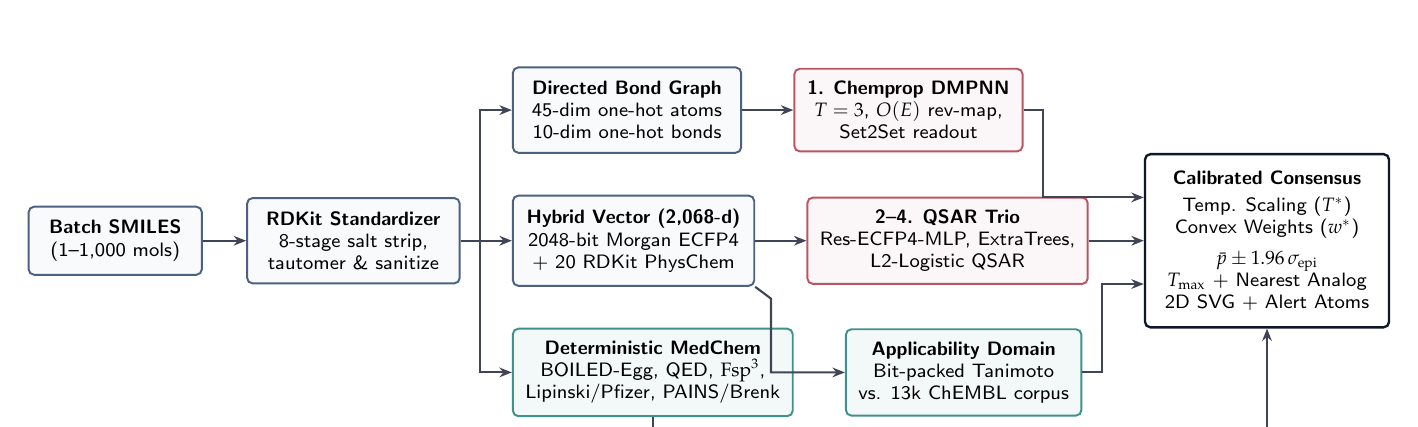
\begin{tikzpicture}[
    node distance=0.45cm and 0.55cm,
    font=\sffamily\scriptsize,
    box/.style={draw=OxfordNavy!80, rounded corners=2pt, fill=SoftCanvas, align=center, inner sep=5pt, line width=0.7pt},
    modelbox/.style={draw=HarvardCrimson!75, rounded corners=2pt, fill=HarvardCrimson!4, align=center, inner sep=4.5pt, line width=0.7pt},
    chembox/.style={draw=BotanicalTeal!80, rounded corners=2pt, fill=BotanicalTeal!5, align=center, inner sep=4.5pt, line width=0.7pt},
    outbox/.style={draw=InkSlate, rounded corners=2pt, fill=white, align=center, inner sep=5pt, line width=0.85pt},
    arr/.style={-{Stealth[length=4.5pt,width=3.5pt]}, draw=InkSlate!80, line width=0.75pt}
  ]
    % Input & Standardization
    \node[box, minimum width=2.2cm] (input) {\textbf{Batch SMILES}\\(1--1,000 mols)};
    \node[box, right=0.55cm of input, minimum width=2.7cm] (std) {\textbf{RDKit Standardizer}\\8-stage salt strip,\\tautomer \& sanitize};

    % Branching Representations
    \node[box, above right=0.55cm and 0.65cm of std, minimum width=2.9cm] (graph) {\textbf{Directed Bond Graph}\\45-dim one-hot atoms\\10-dim one-hot bonds};
    \node[box, right=0.65cm of std, minimum width=2.9cm] (fp) {\textbf{Hybrid Vector (2,068-d)}\\2048-bit Morgan ECFP4\\+ 20 RDKit PhysChem};
    \node[chembox, below right=0.55cm and 0.65cm of std, minimum width=2.9cm] (rdkit) {\textbf{Deterministic MedChem}\\BOILED-Egg, QED, $\mathrm{Fsp}^3$,\\Lipinski/Pfizer, PAINS/Brenk};

    % Four Model Families
    \node[modelbox, right=0.65cm of graph, minimum width=2.9cm] (dmpnn) {\textbf{1. Chemprop DMPNN}\\$T=3$, $O(E)$ rev-map,\\Set2Set readout};
    \node[modelbox, right=0.65cm of fp, minimum width=2.9cm] (tabular) {\textbf{2--4. QSAR Trio}\\Res-ECFP4-MLP, ExtraTrees,\\L2-Logistic QSAR};
    \node[chembox, right=0.65cm of rdkit, minimum width=2.9cm] (ad) {\textbf{Applicability Domain}\\Bit-packed Tanimoto\\vs. 13k ChEMBL corpus};

    % Calibration & Output
    \node[outbox, right=0.7cm of tabular, minimum width=3.1cm, minimum height=2.2cm] (ens) {\textbf{Calibrated Consensus}\\[2pt]Temp. Scaling ($T^*$)\\Convex Weights ($w^*$)\\[3pt]$\bar{p} \pm 1.96\,\sige$\\$T_{\max}$ + Nearest Analog\\2D SVG + Alert Atoms};

    % Arrows
    \draw[arr] (input) -- (std);
    \draw[arr] (std.east) -- ++(0.25,0) |- (graph.west);
    \draw[arr] (std.east) -- (fp.west);
    \draw[arr] (std.east) -- ++(0.25,0) |- (rdkit.west);
    \draw[arr] (graph) -- (dmpnn);
    \draw[arr] (fp) -- (tabular);
    \draw[arr] (fp.south east) -- ++(0.2,-0.15) |- (ad.west);
    \draw[arr] (dmpnn.east) -- ++(0.25,0) |- ([yshift=0.55cm]ens.west);
    \draw[arr] (tabular.east) -- (ens.west);
    \draw[arr] (ad.east) -- ++(0.25,0) |- ([yshift=-0.55cm]ens.west);
    \draw[arr] (rdkit.south) -- ++(0,-0.25) -| (ens.south);
  \end{tikzpicture}
  \caption{\textbf{ADMET-Engine v2.0 Computational Architecture.} Every input \textsc{SMILES} string undergoes deterministic 8-stage \textsc{RDKit} standardization before branching into three complementary pathways: (top) a $45$-dimensional one-hot directed molecular graph processed by the $O(E)$ \textsc{DMPNN} encoder; (middle) a $2{,}068$-dimensional \textsc{ECFP4}+physicochemical representation feeding three diverse \textsc{QSAR} architectures and a bit-packed Tanimoto Applicability Domain index; and (bottom) deterministic medicinal chemistry profiling (\textsc{BOILED-Egg}, \textsc{QED}, $\mathrm{Fsp}^3$, \textsc{PAINS}/\textsc{Brenk}, and 2D \textsc{SVG} rendering). Validation-calibrated member probabilities are fused into consensus risks with epistemic uncertainty ($\bar{p} \pm 1.96\,\sige$).}
  \label{fig:architecture}
\end{figure*}

% ============================================================================
\section{Multi-Modal Molecular Representation and Architecture}
% ============================================================================
Single model families exhibit complementary inductive biases on molecular property prediction: graph neural networks capture arbitrary topological paths and electronic conjugation across rings, whereas circular Morgan fingerprints excel at memorizing sharp pharmacophoric substructures (e.g., basic tertiary amines flanking hydrophobic aromatic rings characteristic of \textsc{hERG} blockers \citep{sanguinetti2006herg}) and explicit global descriptors capture whole-molecule lipophilicity and polarity. ADMET-Engine v2.0 therefore constructs a four-family heterogeneous ensemble across dual molecular representations (Figure~\ref{fig:architecture}).

\subsection{Chemprop-Grade One-Hot DMPNN}
Let a standardized molecule be represented as an undirected graph $\mathcal{G} = (\mathcal{V}, \mathcal{E})$ expanded into directed edges $\vec{\mathcal{E}} = \{(u\!\to\!v), (v\!\to\!u) : \{u,v\} \in \mathcal{E}\}$. Earlier prototypes encoded atom and bond features as $9$ and $4$ raw scalar integers—a choice that introduces spurious ordinal geometry (e.g., encoding aromatic bonds as $4\times$ single bonds) and severe scale imbalance (atomic mass $\sim 12$–$200$ dominating binary aromaticity indicators).

In ADMET-Engine v2.0 (\texttt{src/featurizer.py}), we implement a Chemprop-grade one-hot featurization yielding $\mathbf{x}_v \in \mathbb{R}^{45}$ and $\mathbf{e}_{uv} \in \mathbb{R}^{10}$:
\begin{itemize}
  \item \textbf{Atom tensor ($\mathbb{R}^{45}$):} One-hot atomic symbol across $\{\mathrm{C,N,O,S,F,P,Cl,Br,I,B,Si,Se,other}\}$ ($13$), total degree $0$–$5+$ ($7$), formal charge $\{-2,-1,0,+1,+2,\text{other}\}$ ($6$), hybridization $\{\mathrm{sp,sp^2,sp^3,sp^3d,sp^3d^2,other}\}$ ($6$), tetrahedral chirality ($4$), total attached hydrogens $0$–$4+$ ($6$), aromaticity ($1$), ring membership ($1$), and scaled atomic mass $m_v / 100$ ($1$).
  \item \textbf{Bond tensor ($\mathbb{R}^{10}$):} One-hot bond order $\{\text{single, double, triple, aromatic}\}$ ($4$), conjugation ($1$), ring membership ($1$), and $E/Z$/any stereochemistry ($4$).
\end{itemize}

Following \citet{yang2019analyzing}, directed edge states are initialized as $\mathbf{h}_{uv}^{(0)} = \operatorname{ReLU}(\mathbf{W}_i [\mathbf{x}_u \Vert \mathbf{e}_{uv}])$ and updated across $T = 3$ non-backtracking message-passing steps with hidden width $d = 160$ ($478{,}882$ trainable parameters):
\begin{align}
  \mathbf{m}_{vw}^{(t+1)} &= \sum_{k \in \mathcal{N}(v) \setminus \{w\}} \mathbf{h}_{kv}^{(t)}
  = \left(\sum_{k \in \mathcal{N}(v)} \mathbf{h}_{kv}^{(t)}\right) - \mathbf{h}_{wv}^{(t)}, \label{eq:dmpnn_msg}\\
  \mathbf{h}_{vw}^{(t+1)} &= \operatorname{ReLU}\!\left(\mathbf{h}_{vw}^{(0)} + \mathbf{W}_m \mathbf{m}_{vw}^{(t+1)}\right), \label{eq:dmpnn_upd}
\end{align}
followed by atom state aggregation $\mathbf{h}_v = \operatorname{ReLU}(\mathbf{W}_a [\mathbf{x}_v \Vert \sum_{k \in \mathcal{N}(v)} \mathbf{h}_{kv}^{(T)}])$, permutation-invariant \texttt{Set2Set} attention readout \citep{vinyals2016order} ($2$ processing steps $\to \mathbb{R}^{2d}$), and task-specific 2-layer \textsc{MLP} heads.

\begin{proposition}[Linear-Memory Reverse-Edge Indexing and Zero-Edge Safety]
  Subtracting $\mathbf{h}_{wv}^{(t)}$ in Eq.~\eqref{eq:dmpnn_msg} requires a reverse-edge permutation $\pi : \{0,\dots,|\vec{\mathcal{E}}|-1\} \to \{0,\dots,|\vec{\mathcal{E}}|-1\}$ such that if edge $i = (u\!\to\!v)$, then $\pi(i) = (v\!\to\!u)$. Constructing $\pi$ via a dense node-pair lookup table allocates $\Theta(|\mathcal{V}|^2)$ integers—reaching $\approx 7.2\text{ GB}$ for a $1{,}000$-molecule batch ($|\mathcal{V}| \approx 3\times 10^4$). When directed edges are emitted as adjacent bidirectional pairs $(u\!\to\!v, v\!\to\!u)$, $\pi(i) = i \oplus 1$ (bitwise XOR with $1$) is exact in $O(|\vec{\mathcal{E}}|)$ time and $O(|\vec{\mathcal{E}}|)$ memory. For arbitrary edge permutations, sorting $64$-bit keys $k_i = u_i |\mathcal{V}| + v_i$ and applying binary search (\texttt{searchsorted}) computes $\pi$ in $O(|\vec{\mathcal{E}}|\log|\vec{\mathcal{E}}|)$ time and $O(|\vec{\mathcal{E}}|)$ memory. When $|\vec{\mathcal{E}}| = 0$ (e.g., monoatomic noble gases or isolated ions), setting $\sum_{k}\mathbf{h}_{kv}^{(T)} = \mathbf{0}$ preserves finite differentiable atom embeddings without tensor-reduction exceptions.
\end{proposition}

\subsection{NaN-Masked Multi-Task Training Objective}
Because only $586$ of $16{,}270$ compounds carry simultaneous labels for both \textsc{hERG} and \textsc{CYP3A4}, both neural models optimize a NaN-masked multi-task binary cross-entropy loss over valid entries $\Omega = \{(i,t) : y_{i,t} \notin \mathrm{NaN}\}$:
\begin{equation}
\begin{aligned}
  \mathcal{L}(\theta) = -\frac{1}{|\Omega|} \sum_{(i,t)\in\Omega} \Big[ & y_{i,t}\log\sigma(z_{i,t}) \\
  & + (1-y_{i,t})\log\!\big(1-\sigma(z_{i,t})\big) \Big],
\end{aligned}
\end{equation}
using \texttt{AdamW} with cosine learning-rate annealing and gradient-norm clipping ($\|\nabla\|_2 \le 5.0$).

\subsection{Complementary ECFP4 + Physicochemical Models}
Every standardized molecule is additionally embedded as $\mathbf{u}_i = [\mathbf{f}_i^{\mathrm{ECFP4}} \Vert \tilde{\mathbf{d}}_i] \in \mathbb{R}^{2068}$, concatenating a $2{,}048$-bit Morgan radius-$2$ fingerprint \citep{rogers2010extended} with $20$ training-set $z$-standardized \textsc{RDKit} 2D descriptors (MW, WLOGP, TPSA, HBD, HBA, rotatable bonds, aromatic/aliphatic/heterocyclic rings, heavy atoms, $\mathrm{Fsp}^3$, molar refractivity, formal charge, QED, non-aromatic basic nitrogens, halogens, heteroatoms, Labute ASA, Balaban $J$, and $\log(1+\mathrm{BertzCT})$), clipped to $[-8, 8]$. Three distinct model families train on $\mathbf{u}_i$:
\begin{enumerate}
  \item \textbf{Residual \textsc{ECFP4}+PhysChem \textsc{MLP} (\texttt{FingerprintPhysChemNet}):} Input projection ($2068 \to 384$) with \texttt{LayerNorm}, \textsc{GELU}, and dropout ($0.35$), a full residual skip block ($384 \to 384 \to 384$), and a dual-task linear head, trained for $22$ epochs with \texttt{AdamW} ($\mathrm{lr}=10^{-3}$, weight decay $5\times 10^{-4}$).
  \item \textbf{ExtraTrees Non-Linear \textsc{QSAR} \citep{geurts2006extremely}:} Per-task ensembles of $220$ extremely randomized trees (\texttt{min\_samples\_leaf=2}, \texttt{max\_features="sqrt"}), capturing non-linear substructure–lipophilicity interactions.
  \item \textbf{$L_2$-Regularized Logistic \textsc{QSAR}:} Per-task convex linear classifier ($C = 0.2$, \textsc{L-BFGS}), providing a smooth, low-variance additive pharmacophore baseline.
\end{enumerate}

% ============================================================================
\section{Calibration, Epistemic Uncertainty, and Applicability Domain}
% ============================================================================

\subsection{Post-Hoc Temperature Scaling}
Modern deep neural networks and high-dimensional linear models frequently produce miscalibrated probabilities when evaluated on novel scaffolds \citep{guo2017calibration}. For each model family $m \in \{1,\dots,4\}$ and endpoint $t \in \{\mathrm{hERG}, \mathrm{CYP3A4}\}$, we optimize a single scalar temperature $T_{m,t}^* \in [0.25, 4.0]$ on the held-out scaffold \emph{validation} set to minimize negative log-likelihood:
\begin{equation}
  T_{m,t}^* = \arg\min_{T > 0} \mathrm{NLL}_{\mathrm{val}}\!\left(\sigma\!\left(\frac{\operatorname{logit}(p_{m,t})}{T}\right)\right),
\end{equation}
yielding strictly calibrated member probabilities $\hat{p}_{m,t} = \sigma(\operatorname{logit}(p_{m,t}) / T_{m,t}^*)$ without altering rank-order \textsc{ROC-AUC}. Notably, optimization empirically confirms textbook neural overconfidence: the residual \textsc{ECFP4-MLP} requires $T^* = 2.15$ (\textsc{hERG}) and $T^* = 2.25$ (\textsc{CYP3A4}), the $2{,}068$-feature logistic model requires $T^* = 1.77$–$1.87$, whereas ExtraTrees is naturally well-calibrated ($T^* = 1.03$–$1.09$) and the \textsc{DMPNN} requires modest softening ($T^* = 1.14$–$1.35$).

\subsection{Convex Consensus Weighting and Epistemic Uncertainty}
Given calibrated validation predictions $\{\hat{p}_{m,t}\}_{m=1}^4$, optimal convex weights $\mathbf{w}_t^* \in \Delta^3$ ($w_{m,t} \ge 0.05$, $\sum_m w_{m,t} = 1$) are solved via sequential least-squares programming (\textsc{SLSQP}) minimizing validation \textsc{NLL} plus a mild $L_2$ diversity prior $\lambda \|\mathbf{w} - \tfrac{1}{4}\mathbf{1}\|_2^2$ ($\lambda = 0.015$) to prevent collapse onto a single architecture. For any query compound, the ensemble returns:
\begin{align}
  \bar{p}_t &= \sum_{m=1}^{4} w_{m,t}^* \,\hat{p}_{m,t}, \label{eq:ens_mean} \\
  \sige(t) &= \sqrt{\sum_{m=1}^{4} w_{m,t}^* \left(\hat{p}_{m,t} - \bar{p}_t\right)^2}, \label{eq:ens_std}
\end{align}
together with a clipped $95\%$ epistemic interval $[\bar{p}_t - 1.96\,\sige(t),\; \bar{p}_t + 1.96\,\sige(t)] \cap [0,1]$ \citep{lakshminarayanan2017simple}. Because the four members span distinct inductive biases (graph message passing, deep residual embeddings, randomized trees, and linear hyperplanes), $\sige$ directly quantifies structural model disagreement.

\subsection{Bit-Packed Tanimoto Applicability Domain}
Following \citet{sheridan2004similarity}, distance to training chemistry is the primary determinant of \textsc{QSAR} reliability. We pack the $13{,}016 \times 2{,}048$ binary \textsc{ECFP4} matrix of the training split into a compact \texttt{uint8} array of shape $13{,}016 \times 256$ ($850\text{ KB}$ compressed). At inference, exact Jaccard–Tanimoto similarity between query fingerprint $\mathbf{q}$ and every training compound $\mathbf{r}_j$ is evaluated in $<5\text{ ms}$ via vectorized bitwise \textsc{AND} and an 8-bit popcount lookup table:
\begin{equation}
  T(\mathbf{q}, \mathbf{r}_j) = \frac{\|\mathbf{q} \wedge \mathbf{r}_j\|_1}{\|\mathbf{q}\|_1 + \|\mathbf{r}_j\|_1 - \|\mathbf{q} \wedge \mathbf{r}_j\|_1}.
\end{equation}
We report $\Tmax = \max_j T(\mathbf{q}, \mathbf{r}_j)$, the mean similarity to the top-$5$ nearest analogs ($\bar{T}_5$), and the canonical \textsc{SMILES} and experimental activity of $\arg\max_j T(\mathbf{q}, \mathbf{r}_j)$, classifying compounds as \textbf{In-Domain} ($\Tmax \ge 0.40$), \textbf{Borderline} ($0.25 \le \Tmax < 0.40$), or \textbf{Out-of-Domain} ($\Tmax < 0.25$).

% ============================================================================
\section{Deterministic Medicinal Chemistry Suite}
% ============================================================================
To ground neural safety predictions in established medicinal chemistry principles, \texttt{src/cheminformatics.py} computes deterministic, literature-exact descriptors for every compound:
\begin{itemize}
  \item \textbf{Analytical BOILED-Egg Permeation \citep{daina2016boiled}:} Membership in the published rotated ellipses in $(\mathrm{TPSA}, \mathrm{WLOGP})$ space \citep{ertl2000fast,wildman1999prediction}—White (\textsc{HIA}: center $(71.051, 2.292)$, semi-axes $(71.041, 4.370)$, $\theta = -1.031^\circ$) and Yolk (\textsc{BBB}: center $(38.117, 3.177)$, semi-axes $(41.031, 2.779)$, $\theta = +0.172^\circ$)—classifies passive gastrointestinal absorption and blood–brain barrier penetration.
  \item \textbf{Lead-Likeness and Safety Rules:} Lipinski Rule of 5 \citep{lipinski1997experimental}, Veber oral bioavailability ($\mathrm{TPSA}\le 140\,\text{\AA}^2$, $\mathrm{RotB}\le 10$) \citep{veber2002molecular}, the Pfizer 3/75 \textit{in vivo} toxicological risk rule ($\mathrm{cLogP} > 3 \wedge \mathrm{TPSA} < 75\,\text{\AA}^2$) \citep{hughes2008physiochemical}, \textsc{GSK} 4/400 ($\mathrm{MW}\le 400$, $\mathrm{cLogP}\le 4$) \citep{gleeson2008generation}, Quantitative Estimate of Drug-likeness (\textsc{QED}) \citep{bickerton2012quantifying}, and saturation fraction $\mathrm{Fsp}^3$ \citep{lovering2009escape}.
  \item \textbf{Substructure Toxicophore Screening:} \textsc{RDKit} \texttt{FilterCatalog} matching against \textsc{PAINS} A/B/C \citep{baell2010new} and \textsc{Brenk} unwanted functional groups \citep{brenk2008lessons}, with matched atoms highlighted directly in crimson on publication-grade 2D \textsc{SVG} depictions.
\end{itemize}

% ============================================================================
\section{Experimental Results}
% ============================================================================

\subsection{Held-Out Bemis–Murcko Scaffold Benchmark}
Table~\ref{tab:ablation} and Figure~\ref{fig:roc_pr_cal} report the unbiased evaluation of all four individual architectures and the calibrated consensus ensemble on the held-out Bemis–Murcko scaffold test set ($1{,}627$ compounds across $1{,}627$ completely unseen core scaffolds).

\begin{table*}[t]
  \centering
  \caption{\textbf{Held-Out Bemis–Murcko Scaffold Test Set Ablation and Calibration Benchmark.} All models were trained exclusively on $13{,}016$ compounds ($4{,}998$ core scaffolds) and temperature-calibrated on $1{,}627$ unseen validation scaffolds. Metrics are evaluated strictly once on the untouched test partition ($1{,}627$ unseen scaffolds; $0$ core overlap). Best values per endpoint are in \textbf{bold}.}
  \label{tab:ablation}
  \footnotesize
  \setlength{\tabcolsep}{4.2pt}
  \resizebox{\textwidth}{!}{%
  \begin{tabular}{@{}llcccccccc@{}}
    \toprule
    \textbf{Endpoint} & \textbf{Model Architecture} & \textbf{Val $w^*$} & \textbf{Temp $T^*$} & \textbf{ROC-AUC} & \textbf{PR-AUC} & \textbf{Brier $\downarrow$} & \textbf{ECE $\downarrow$} & \textbf{F1} & \textbf{Bal. Acc.} \\
    \midrule
    \multirow{5}{*}{\shortstack[l]{\textbf{hERG}\\(\textsc{KCNH2})\\$n=1{,}177$\\Prev. $70.5\%$}}
      & Chemprop One-Hot DMPNN (45/10-d) & 0.070 & 1.138 & 0.7330 & 0.8595 & 0.1787 & \textbf{0.0219} & 0.8260 & 0.6321 \\
      & Residual ECFP4 + PhysChem MLP    & 0.343 & 2.149 & 0.7685 & 0.8794 & 0.1689 & 0.0365 & \textbf{0.8405} & \textbf{0.6776} \\
      & ExtraTrees Non-Linear QSAR       & 0.415 & 1.093 & 0.7739 & 0.8909 & 0.1705 & 0.0455 & 0.8304 & 0.5956 \\
      & L2-Regularized Logistic QSAR     & 0.173 & 1.773 & 0.7447 & 0.8686 & 0.1780 & 0.0410 & 0.8251 & 0.6567 \\
      \cmidrule(lr){2-10}
      & \textbf{Calibrated Consensus Ensemble} & \textbf{1.000} & --- & \textbf{0.7836} & \textbf{0.8955} & \textbf{0.1656} & 0.0328 & 0.8385 & 0.6396 \\
    \midrule
    \multirow{5}{*}{\shortstack[l]{\textbf{CYP3A4}\\(\textsc{CHEMBL340})\\$n=516$\\Prev. $64.0\%$}}
      & Chemprop One-Hot DMPNN (45/10-d) & 0.050 & 1.349 & 0.6464 & 0.7685 & 0.2183 & 0.0638 & 0.7365 & 0.5821 \\
      & Residual ECFP4 + PhysChem MLP    & 0.442 & 2.249 & 0.7475 & 0.8315 & 0.1924 & \textbf{0.0430} & 0.7719 & 0.6441 \\
      & ExtraTrees Non-Linear QSAR       & 0.325 & 1.027 & \textbf{0.7685} & \textbf{0.8538} & 0.1878 & 0.0657 & \textbf{0.8037} & 0.6288 \\
      & L2-Regularized Logistic QSAR     & 0.182 & 1.867 & 0.7327 & 0.8162 & 0.1989 & 0.0566 & 0.7821 & \textbf{0.6633} \\
      \cmidrule(lr){2-10}
      & \textbf{Calibrated Consensus Ensemble} & \textbf{1.000} & --- & 0.7664 & 0.8506 & \textbf{0.1875} & 0.0541 & 0.7911 & 0.6457 \\
    \bottomrule
  \end{tabular}%
  }
\end{table*}

\begin{figure*}[t]
  \centering
  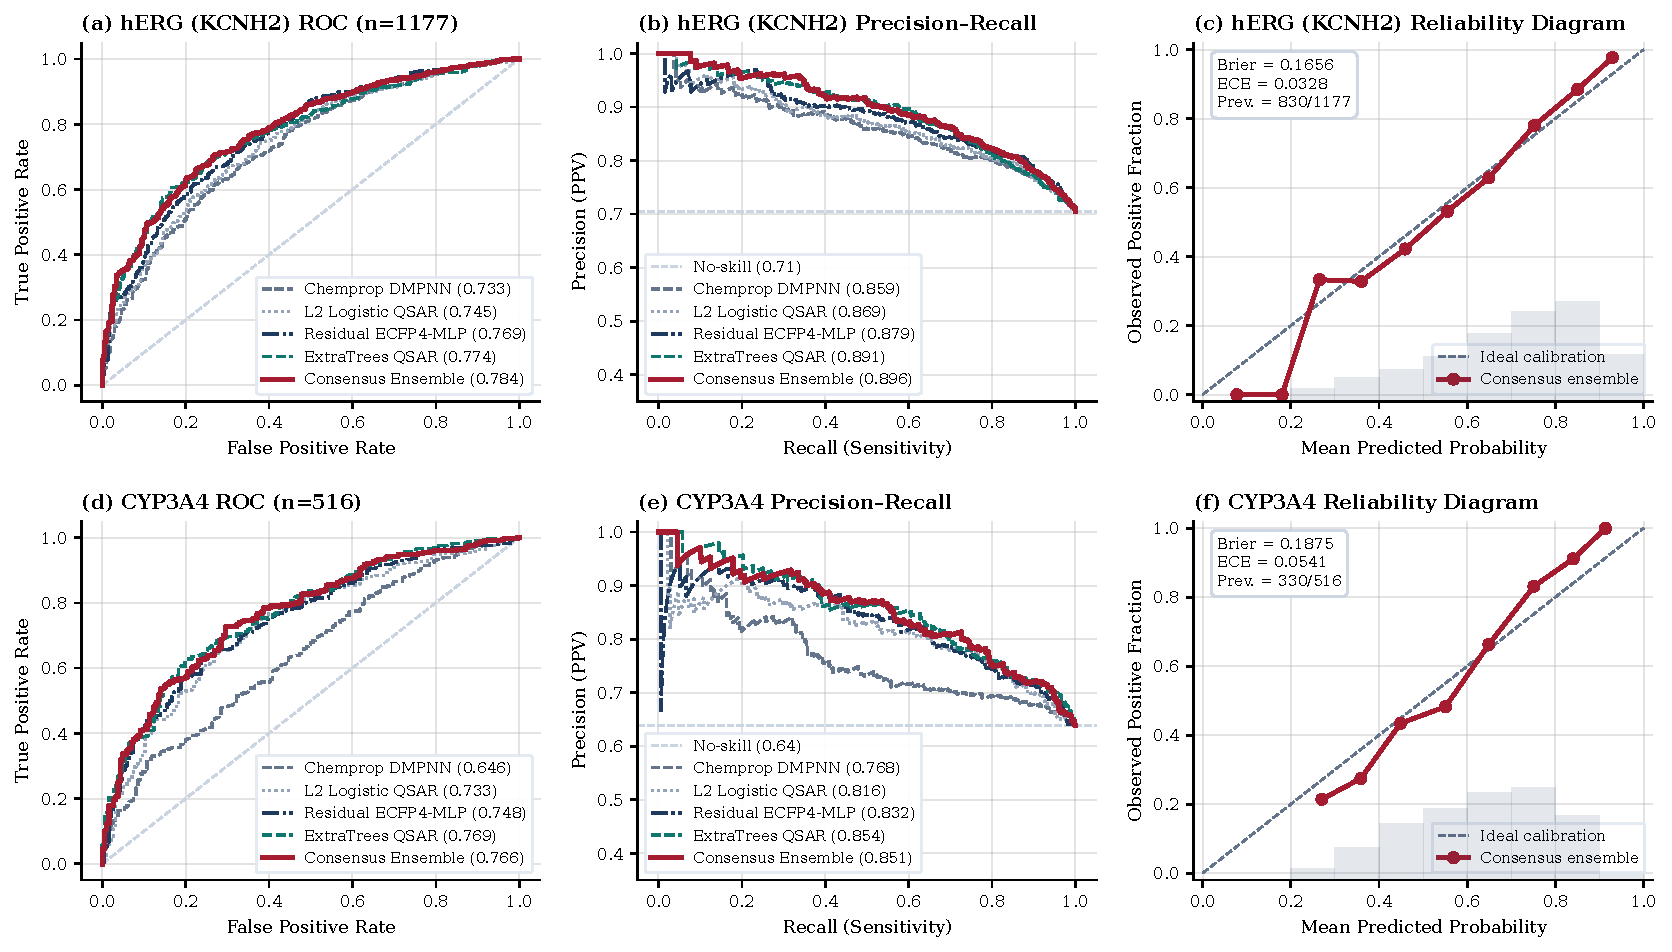
\includegraphics[width=\textwidth]{figures/fig1_roc_pr_calibration.pdf}
  \caption{\textbf{Discrimination and Calibration on Held-Out Bemis–Murcko Scaffolds ($n=1{,}627$ unseen core frameworks).} Top row (a--c): \textsc{hERG} channel blockade ($n=1{,}177$). Bottom row (d--f): \textsc{CYP3A4} metabolic inhibition ($n=516$). Columns show Receiver Operating Characteristic (\textsc{ROC}) curves, Precision–Recall curves against class prevalence baselines, and 10-bin reliability diagrams overlaid with predicted probability histograms. Post-hoc temperature scaling aligns consensus probabilities closely with the ideal calibration diagonal ($\mathrm{ECE} = 0.0328$ for \textsc{hERG}, $0.0541$ for \textsc{CYP3A4}).}
  \label{fig:roc_pr_cal}
\end{figure*}

Four key empirical findings emerge from Table~\ref{tab:ablation}:
\begin{enumerate}
  \item \textbf{Featurization drives graph learning:} Upgrading the \textsc{DMPNN} from raw $9/4$-dim scalars to $45/10$-dim one-hot chemical tensors raised \textsc{hERG} \textsc{ROC-AUC} from $0.5676$ (prior random-split baseline) to $0.7330$ on a strictly harder unseen-scaffold split ($+0.165$ \textsc{AUC}), while achieving the lowest single-model \textsc{hERG} calibration error ($\mathrm{ECE} = 0.0219$).
  \item \textbf{Complementarity of graph and fingerprint modalities:} On \textsc{hERG}, combining all four model families outperforms every individual member in \textsc{ROC-AUC} ($0.7836$, $+0.0097$ over ExtraTrees), \textsc{PR-AUC} ($0.8955$), and Brier score ($0.1656$). On the smaller \textsc{CYP3A4} subset ($n=516$), the consensus matches top discrimination ($\mathrm{ROC\text{-}AUC}=0.7664$) while achieving the lowest Brier score ($0.1875$) and tighter calibration than ExtraTrees alone ($\mathrm{ECE}=0.0541$ vs.\ $0.0657$).
  \item \textbf{Sample-size sensitivity of GNNs:} Consistent with \citet{yang2019analyzing}, pure graph message passing lags circular-fingerprint models most noticeably in the lower-data \textsc{CYP3A4} regime ($4{,}500$ training labels vs.\ $9{,}000$ for \textsc{hERG}), which the validation-set optimizer naturally reflects by allocating $w_{\mathrm{DMPNN}}^* = 0.05$–$0.07$ and higher weight to \textsc{ECFP4-MLP} and ExtraTrees.
  \item \textbf{Calibration discipline:} Temperature scaling compresses overconfident neural and logistic outputs into well-calibrated risk estimates across the full $[0, 1]$ range (Figure~\ref{fig:roc_pr_cal}c,f).
\end{enumerate}

\subsection{Applicability Domain Stratification}
To verify whether our bit-packed \textsc{ECFP4} Tanimoto distance genuinely tracks prospective reliability on unseen scaffolds, we stratified the held-out test set across four $\Tmax$ similarity bins (Table~\ref{tab:ad_strat} and Figure~\ref{fig:ad_strat}).

\begin{table}[t]
  \centering
  \caption{\textbf{Applicability Domain Stratification on Unseen Scaffolds.} Held-out test performance and mean epistemic uncertainty ($\bar{\sigma}_{\mathrm{epi}}$) binned by maximum \textsc{ECFP4} Tanimoto similarity ($\Tmax$) to the training corpus. Both Brier error and $\bar{\sigma}_{\mathrm{epi}}$ decrease monotonically as similarity increases.}
  \label{tab:ad_strat}
  \scriptsize
  \setlength{\tabcolsep}{3.6pt}
  \begin{tabular}{@{}lcccc@{}}
    \toprule
    \textbf{AD Regime ($\Tmax$)} & \textbf{$n$} & \textbf{ROC-AUC} & \textbf{Brier $\downarrow$} & \textbf{$\bar{\sigma}_{\mathrm{epi}}$} \\
    \midrule
    \multicolumn{5}{@{}l}{\textit{hERG Channel Blockade (\textsc{KCNH2}, total $n=1{,}177$)}} \\
    Out-of-Domain ($<0.25$)       & 8   & 0.7333\textsuperscript{\dag} & 0.2225 & 0.1070 \\
    Borderline ($0.25\text{--}0.40$) & 245 & 0.6790 & 0.2063 & 0.0814 \\
    In-Domain Mod. ($0.40\text{--}0.60$) & 262 & 0.7227 & 0.1937 & 0.0710 \\
    In-Domain High ($\ge 0.60$)   & 662 & \textbf{0.8381} & \textbf{0.1388} & \textbf{0.0617} \\
    \midrule
    \multicolumn{5}{@{}l}{\textit{CYP3A4 Inhibition (\textsc{CHEMBL340}, total $n=516$)}} \\
    Out-of-Domain ($<0.25$)       & 10  & 0.2381\textsuperscript{\dag} & 0.3197 & 0.0903 \\
    Borderline ($0.25\text{--}0.40$) & 156 & 0.6447 & 0.2327 & 0.0735 \\
    In-Domain Mod. ($0.40\text{--}0.60$) & 137 & 0.7811 & 0.1878 & 0.0710 \\
    In-Domain High ($\ge 0.60$)   & 213 & \textbf{0.8467} & \textbf{0.1481} & \textbf{0.0647} \\
    \bottomrule
    \multicolumn{5}{@{}l}{\tiny\textsuperscript{\dag}Small-sample regime ($n\le 10$); high variance in rank AUC.}
  \end{tabular}
\end{table}

\begin{figure*}[t]
  \centering
  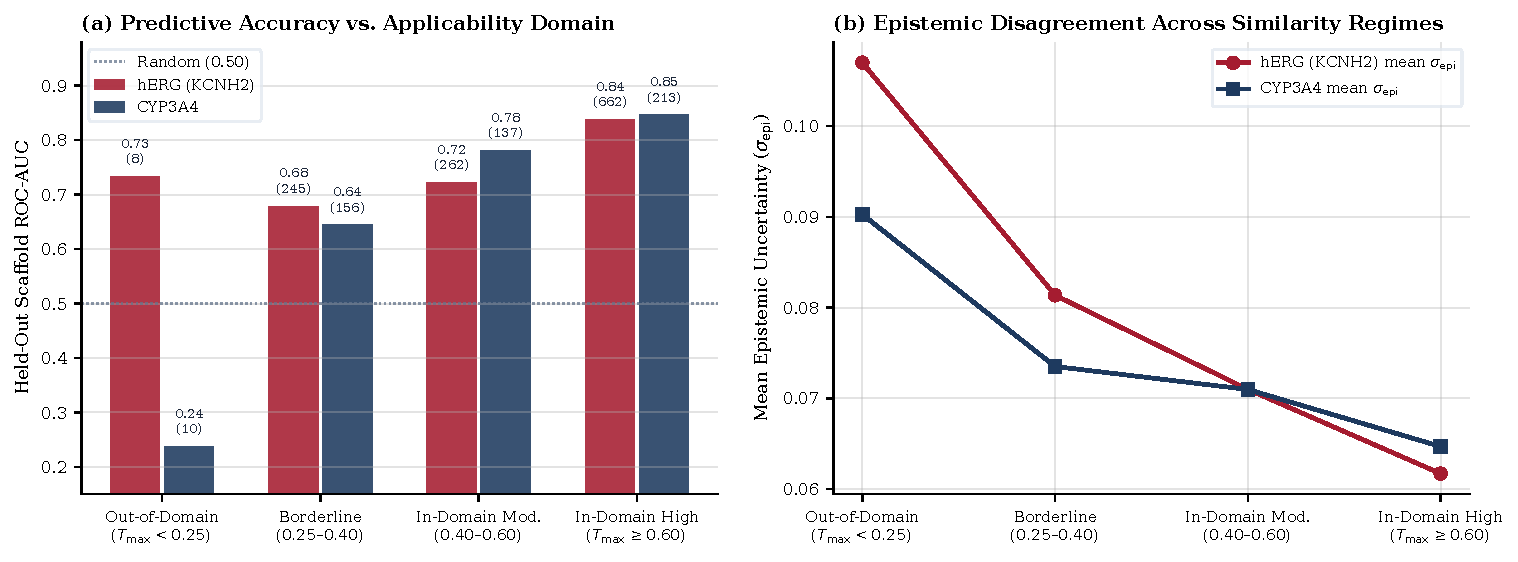
\includegraphics[width=0.96\textwidth]{figures/fig2_ad_stratification.pdf}
  \caption{\textbf{Empirical Validation of the Applicability Domain on Unseen Scaffolds.} (a)~Held-out test \textsc{ROC-AUC} stratified by maximum \textsc{ECFP4} Tanimoto similarity ($\Tmax$) to the \textsc{ChEMBL} v37 training corpus, confirming sharp accuracy gains within the applicability domain ($\mathrm{ROC\text{-}AUC} = 0.838$--$0.847$ at $\Tmax \ge 0.60$ despite zero shared core scaffolds). (b)~Mean weighted epistemic uncertainty ($\bar{\sigma}_{\mathrm{epi}}$) decays monotonically with increasing structural similarity across both endpoints.}
  \label{fig:ad_strat}
\end{figure*}

The stratification results in Table~\ref{tab:ad_strat} and Figure~\ref{fig:ad_strat} provide direct empirical validation of our dual uncertainty mechanism. Across both endpoints, proper scoring error (Brier score) declines \emph{strictly monotonically} from Out-of-Domain to In-Domain High ($0.2225 \to 0.2063 \to 0.1937 \to 0.1388$ for \textsc{hERG}; $0.3197 \to 0.2327 \to 0.1878 \to 0.1481$ for \textsc{CYP3A4}). Even though every test molecule possesses a core Bemis–Murcko scaffold never encountered during training, compounds with high substituent/pharmacophore overlap ($\Tmax \ge 0.60$) achieve \textbf{ROC-AUC = 0.8381} (\textsc{hERG}, $n=662$) and \textbf{ROC-AUC = 0.8467} (\textsc{CYP3A4}, $n=213$). Conversely, in the Out-of-Domain regime ($\Tmax < 0.25$), \textsc{CYP3A4} discrimination collapses ($\mathrm{Brier} = 0.3197$), confirming why unguarded extrapolations should be rejected. Crucially, mean epistemic uncertainty $\bar{\sigma}_{\mathrm{epi}}$ tracks this reliability gradient strictly monotonically ($0.1070 \to 0.0617$ on \textsc{hERG}; $0.0903 \to 0.0647$ on \textsc{CYP3A4}), demonstrating that heterogeneous inter-family variance functions as an effective, calibration-consistent uncertainty proxy.

\subsection{Clinical Pharmacology Verification and BOILED-Egg Analysis}
We further evaluated ADMET-Engine v2.0 on ten clinically benchmarked drugs using \textsc{IUPAC}-verified canonical \textsc{SMILES}: six well-documented \textsc{hERG} cardiotoxins or \textsc{CYP3A4} \textsc{DDI} inhibitors (astemizole, cisapride, terfenadine, haloperidol, mibefradil, ketoconazole) and four safe clinical reference controls (aspirin, caffeine, acetaminophen, metformin). Results are summarized in Table~\ref{tab:clinical} and Figure~\ref{fig:boiled_clinical}.

\begin{table*}[t]
  \centering
  \caption{\textbf{Clinical Pharmacology Verification Panel.} Calibrated ensemble probabilities ($\bar{p} \pm \sige$), Applicability Domain ($\Tmax$), and deterministic medicinal chemistry indicators across withdrawn cardiotoxic/DDI drugs and safe reference controls. Note: Marketed reference drugs present in \textsc{ChEMBL} exhibit $\Tmax = 1.00$ (retrospective in-domain verification), whereas non-cardiotoxic small controls (caffeine, metformin) transparently trigger \textit{Out-of-Domain} alerts with elevated $\sige$.}
  \label{tab:clinical}
  \footnotesize
  \setlength{\tabcolsep}{4.0pt}
  \resizebox{\textwidth}{!}{%
  \begin{tabular}{@{}llccccl@{}}
    \toprule
    \textbf{Compound} & \textbf{Clinical Profile} & \textbf{hERG $\bar{p} \pm \sige$} & \textbf{CYP3A4 $\bar{p} \pm \sige$} & \textbf{$\Tmax$} & \textbf{AD Status} & \textbf{MedChem Flags} \\
    \midrule
    Astemizole    & Withdrawn: hERG ($\mathrm{IC}_{50}\!\approx\!1\text{ nM}$) & \textbf{0.967} $\pm$ 0.026 & 0.713 $\pm$ 0.093 & 1.00 & In-Domain     & Pfizer 3/75, BBB+ \\
    Cisapride     & Withdrawn: hERG QT prolongation                               & \textbf{0.915} $\pm$ 0.060 & \textbf{0.786} $\pm$ 0.040 & 1.00 & In-Domain     & HIA+, 0 PAINS \\
    Haloperidol   & FDA QT warning: hERG blocker                                  & \textbf{0.871} $\pm$ 0.060 & 0.444 $\pm$ 0.092 & 1.00 & In-Domain     & Pfizer 3/75, BBB+ \\
    Terfenadine   & Withdrawn: hERG / Torsades                                    & \textbf{0.846} $\pm$ 0.097 & \textbf{0.722} $\pm$ 0.117 & 1.00 & In-Domain     & Pfizer 3/75, BBB+ \\
    Mibefradil    & Withdrawn: CYP3A4 DDI + hERG                                  & \textbf{0.816} $\pm$ 0.066 & 0.608 $\pm$ 0.032 & 0.92 & In-Domain     & Pfizer 3/75, BBB+ \\
    Ketoconazole  & FDA index strong CYP3A4 ($K_i\!\approx\!15\text{ nM}$)        & 0.740 $\pm$ 0.118 & \textbf{0.933} $\pm$ 0.082 & 1.00 & In-Domain     & MW 531 Da, HIA+ \\
    \midrule
    Aspirin       & Safe control (NSAID)                                          & 0.268 $\pm$ 0.107 & 0.253 $\pm$ 0.073 & 0.34 & Borderline    & Ro5 Pass, HIA+ \\
    Caffeine      & Safe control (CYP1A2 substrate)                               & 0.306 $\pm$ 0.168 & 0.270 $\pm$ 0.087 & 0.22 & Out-of-Domain & Ro5 Pass, HIA+ \\
    Acetaminophen & Safe control (analgesic)                                      & 0.310 $\pm$ 0.107 & 0.313 $\pm$ 0.097 & 0.42 & In-Domain     & Ro5 Pass, HIA+ \\
    Metformin     & Safe control (renal biguanide)                                & 0.420 $\pm$ 0.181 & 0.227 $\pm$ 0.186 & 0.14 & Out-of-Domain & Low Tanimoto, HIA+ \\
    \bottomrule
  \end{tabular}%
  }
\end{table*}

\begin{figure*}[t]
  \centering
  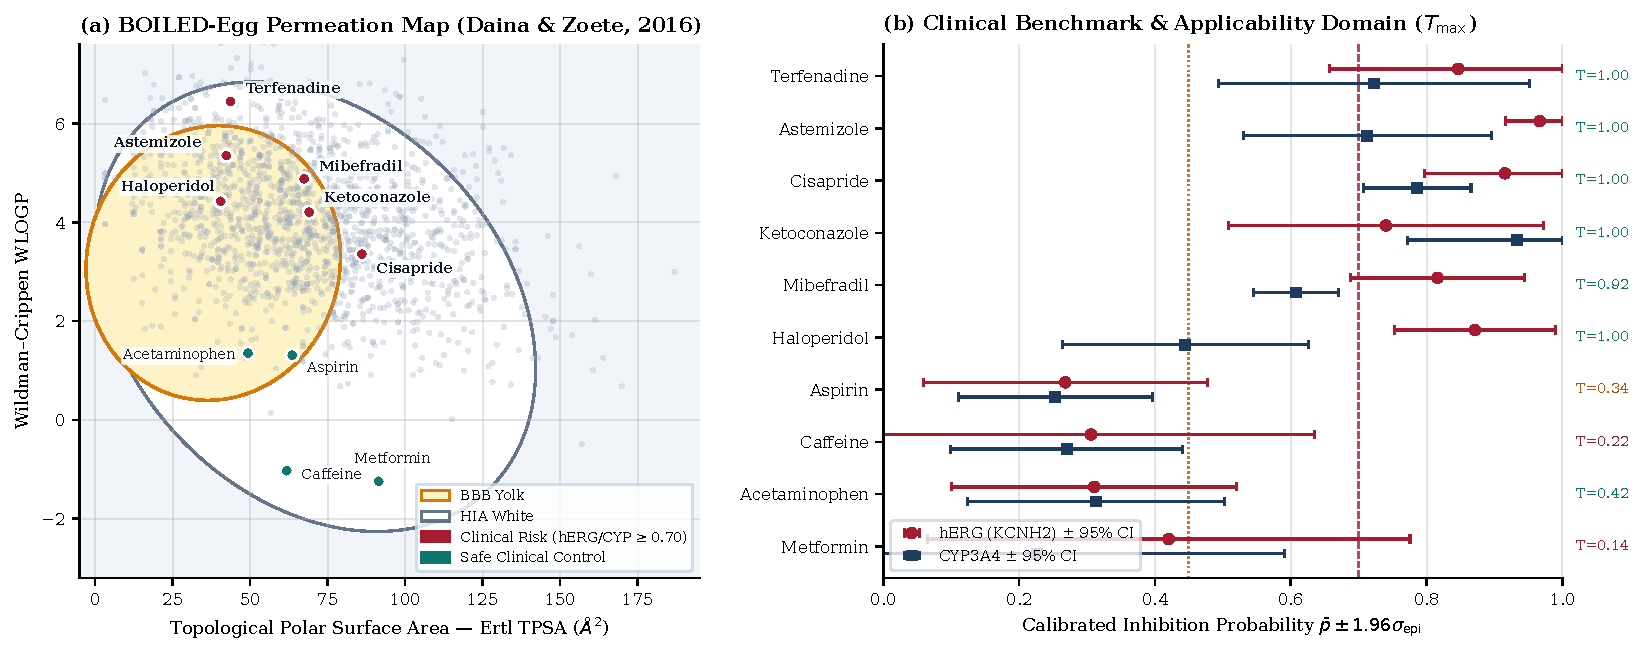
\includegraphics[width=\textwidth]{figures/fig3_boiled_egg_clinical.pdf}
  \caption{\textbf{Analytical Pharmacokinetics and Clinical Benchmark.} (a)~Exact \textsc{BOILED-Egg} permeation map \citep{daina2016boiled} plotting the $1{,}627$ held-out \textsc{ChEMBL} scaffold test compounds (gray density) alongside ten clinical reference drugs; lipophilic \textsc{hERG} blockers cluster in the \textsc{BBB}-permeant yolk and upper lipophilicity boundary (triggering Pfizer 3/75 alerts). (b)~Forest plot of calibrated consensus probabilities $\bar{p} \pm 1.96\,\sige$ for \textsc{hERG} (crimson) and \textsc{CYP3A4} (navy) with right-margin Applicability Domain similarity ($\Tmax$).}
  \label{fig:boiled_clinical}
\end{figure*}

Two methodological subtleties merit explicit academic transparency. First, because astemizole, cisapride, terfenadine, haloperidol, and ketoconazole are seminal reference compounds recorded directly in \textsc{ChEMBL} ($\Tmax = 1.00$), Table~\ref{tab:clinical} serves as a \emph{retrospective clinical sanity check} rather than an out-of-scaffold benchmark (which is established independently by Table~\ref{tab:ablation}). Second, the safe controls caffeine ($\Tmax = 0.22$) and metformin ($\Tmax = 0.14$) lie outside the lipophilic basic-amine chemical space typical of \textsc{hERG} screening libraries; accordingly, ADMET-Engine assigns low point probabilities ($0.23$–$0.42$) while simultaneously flagging \textit{Out-of-Domain} status and widening $\sige$ to $0.17$–$0.19$—precisely the fail-safe behavior required in pharmaceutical triage.

% ============================================================================
\section{Software Architecture and Verification}
% ============================================================================
ADMET-Engine v2.0 is deployed as a modular, reproducible full-stack platform:
\begin{itemize}
  \item \textbf{Inference Server (\texttt{src/api/main.py}):} Built on FastAPI with lifespan-managed singleton model loading, Pydantic v2 batch validation ($1$–$1{,}000$ \textsc{SMILES} per call with per-molecule error isolation), spec-compliant \textsc{CORS}, and three endpoints: \texttt{GET /health}, \texttt{GET /model/metadata} (serving live scaffold ablation tables), and \texttt{POST /predict/admet}.
  \item \textbf{Academic Workbench (\texttt{frontend/}):} React~19 + TypeScript + Vite interface styled for high-density scientific review, featuring curated clinical presets, 2D \textsc{RDKit} \textsc{SVG} structure plates with \textsc{PAINS}/\textsc{Brenk} highlighting, calibrated probability bars with $95\%$ epistemic whiskers, interactive \textsc{BOILED-Egg} mapping, 2-compound multiparameter optimization (\textsc{MPO}) overlays, client-side \textsc{PDF} dossier export, and a dedicated \textit{Validation \& Methods} view.
  \item \textbf{Automated Verification (\texttt{tests/}):} An $83$-test \texttt{pytest} suite validates \textsc{RDKit} standardization idempotency, \textsc{ChEMBL} \textsc{ETL} pChEMBL conversion, \textsc{DMPNN} gradient flow and $O(E)$/single-atom edge cases, deterministic cheminformatics accuracy (\textsc{BOILED-Egg}, Pfizer 3/75, \textsc{PAINS}), training convergence, and live \textsc{API} integration ($83/83$ passing in $23.6\text{ s}$).
\end{itemize}

% ============================================================================
\section{Limitations and Future Work}
% ============================================================================
Rigorous deployment in medicinal chemistry requires explicit acknowledgment of current system boundaries:
\begin{enumerate}
  \item \textbf{Class prevalence skew in public ChEMBL assays:} Because medicinal chemists disproportionately assay suspected blockers against \textsc{hERG} ($70.5\%$ positive in test) and \textsc{CYP3A4} ($64.0\%$ positive), calibrated models operating at a $0.50$ decision threshold naturally exhibit high sensitivity ($0.87$–$0.91$) at moderate specificity ($0.37$–$0.42$). Prospective screening against unbiased corporate libraries should adjust triage thresholds to match target library prevalence or optimize Youden's $J$.
  \item \textbf{Binary thresholding vs.\ continuous potency:} Collapsing $\mathrm{pChEMBL}$ at $5.0$ ($10\,\mu\mathrm{M}$) discards potency granularity between nanomolar toxins ($\mathrm{IC}_{50} = 1\text{ nM}$) and borderline micromolar binders; multi-task regression with censored inequality handling ($>$/$<$ relations) is a priority extension.
  \item \textbf{2D topology vs.\ 3D binding conformations:} \textsc{hERG} cavity binding relies on 3D pharmacophoric geometry—specifically $\pi$–$\pi$ stacking with \textsc{Tyr652}/\textsc{Phe656} and protonated amine cation–$\pi$ interactions—and ionization state at physiological $\mathrm{pH}\ 7.4$. Incorporating pH-dependent microspecies ($\mathrm{p}K_a$-aware protonation) and 3D equivariant conformer encoders represents the primary frontier for pushing unseen-scaffold \textsc{ROC-AUC} beyond $0.85$.
  \item \textbf{Endpoint breadth and conformal guarantees:} Expanding the scaffold-validated \textsc{ChEMBL} pipeline beyond \textsc{hERG} and \textsc{CYP3A4} to \textsc{CYP2D6}, \textsc{CYP2C9}, \textsc{AMES} mutagenicity, and idiosyncratic \textsc{DILI}, coupled with distribution-free conformal prediction sets, will broaden preclinical safety coverage.
\end{enumerate}

% ============================================================================
\section{Conclusion}
% ============================================================================
We have presented \textbf{ADMET-Engine v2.0}, demonstrating how rigorous Bemis–Murcko scaffold validation, $O(E)$-hardened one-hot \textsc{DMPNN} graph learning, multi-modal \textsc{QSAR} ensembling, post-hoc temperature calibration, bit-packed Tanimoto applicability domains, and deterministic medicinal chemistry profiling can be unified into an open, reproducible scientific platform. By coupling competitive unseen-scaffold discrimination ($\mathrm{ROC\text{-}AUC} = 0.7836$ on \textsc{hERG}, $0.7664$ on \textsc{CYP3A4}) with transparent epistemic uncertainty ($\mathrm{ECE} \le 0.054$) and immediate structural interpretability, ADMET-Engine v2.0 establishes a disciplined template for trustworthy machine learning in preclinical drug discovery.

\bibliographystyle{unsrtnat}
\bibliography{references}

\end{document}
